\documentclass{MO824}
\usepackage[utf8]{inputenc}
\usepackage[brazil]{babel}      % para texto em Português
\usepackage{amsmath,amssymb}
\usepackage{hyperref}
\usepackage{subfig}
\usepackage{tikzit}
\usepackage{hyphenat}
\input{sample.tikzstyles}
\newcommand{\Z}{\mathbb{Z}}
\newcommand{\N}{\mathbb{N}}
\usepackage[ruled, portuguese, onelanguage]{algorithm2e}
\usepackage{algorithmic}

\title{Avaliando Mateurísticas e Modelos Matemáticos para o Problema dos Brigadistas}

\author{
    Eduardo Barros Innarelli - RA 170161\\
    Victor Ferreira Ferrari  - RA 187890\\
}

\begin{document}

\criartitulo

\runningheads{E.B. Innarelli e V.F. Ferrari}%
{Projeto Final}

\begin{abstract}
{\bf Resumo}. Este trabalho consiste de uma exploração do Problema dos Brigadistas, ou Firefighter Problem, com a implementação de técnicas comuns em pesquisa operacional e otimização combinatória. A principal técnica implementada é a descrita em Ramos et al. \cite{natanael,nat_dissertation}, que consiste de uma mateurística inspirada no GRASP, com busca local adaptativa em um \textit{pool} de soluções gulosas aleatorizadas, e uma estratégia de intensificação aplicada na melhor solução encontrada. A busca local consiste na fixação de variáveis de uma $k$-vizinhança de uma solução base, e da resolução de um modelo matemático do subproblema criado por essa fixação. Além disso, foram implementados dois modelos matemáticos inteiros no \textit{solver} Gurobi, sendo um clássico e outro alterado com fixação de variáveis e agregação de restrições. Os métodos foram executados com o melhor conjunto de parâmetros encontrado no trabalho original e testados com um subconjunto de 22 instâncias dos conjuntos disponibilizados por Ramos et al. \cite{ffp-instances-page}. O experimento foi um sucesso, com boas soluções encontradas tanto pelos modelos quanto pela mateurística, e um desempenho comparável, se levemente inferior, à implementação de referência de Ramos et al. No futuro, outras metaheurísticas podem seguir alguns dos conceitos propostos, como Busca Tabu e \textit{Simulated Annealing}.

{\bf Palavras-chave}. Firefighter, Grafos, GRASP, metaheurística, mateurística.

\end{abstract}

\section{Introdução}
    O objeto de estudo deste projeto é o Problema dos Brigadistas (do inglês Firefighter Problem, abreviado como FFP), inicialmente proposto por Bert Hartnell em 1995 \cite{original}. O FFP modela de modo determinístico e discreto no tempo a propagação de fogo em uma área, representada por um grafo $G$.
    
    Informalmente, suponha que um bombeiro possa evitar com que o fogo de um vértice incendiado se espalhe para um vizinho não-incendiado, e que há um número fixo de bombeiros disponíveis em cada instante de tempo. Assuma, também, que a partir do momento que um vértice é queimado ou defendido ele assim permanecerá até o fim da propagação do fogo em todo o grafo. No início, um incêndio se inicia em um conjunto dos vértices de $G$ e deve-se decidir em quais dos vértices do grafo alocar os bombeiros. O fogo se alastra, então, para todos seus vizinhos não-incendiados e desprotegidos, e o processo se repete até o momento em que nenhum vértice possa ser queimado.
    
    A \figurename~\ref{fig:exemplo} ilustra um caso em que o fogo se origina no vértice 1 e há apenas um bombeiro disponível por instante de tempo. Os vértices queimados são identificados em vermelho, os defendidos diretamente pelo bombeiro em verde e os salvos indiretamente (vértices que o fogo não consegue alcançar) em azul. Note como a escolha de proteger o vértice 2 na primeira iteração diminuiu o impacto do incêndio. A solução ilustrada é ótima para a instância.

    \begin{figure}
    \ctikzfig{ffp}
    \caption{Exemplo de 2 iterações do FFP}
    \label{fig:exemplo}
    \end{figure}
    
    Ainda que o modelo descrito represente a propagação e contenção de fogo em um grafo, é imediato adaptá-lo para que reflita outros cenários de espalhamento de agentes nocivos, tais como vírus em redes de computadores e epidemias em regiões geográficas. 
    
    Naturalmente, é desejável proteger o maior número de vértices possível desses agentes e as soluções adotadas como base deste projeto visam otimizar essa quantidade, mas há uma série de outros objetivos que podem ser derivados do modelo: minimizar o número de unidades de tempo até que a propagação acabe, determinar se todos os vértices de um conjunto específico podem ser protegidos, encontrar o número necessário de entidades (bombeiros, se tratando do FFP) necessárias para salvar um número, fração ou subconjunto dos vértices, entre outros. Por conta dessa flexibilidade e da relevância pública dos cenários que modela, consideramos o FFP um problema interessante de se estudar neste trabalho.

\subsection{O Problema dos Brigadistas}
    \subsubsection{Definição}
    Seja $G=(V,E)$ um grafo não-ponderado e não-direcionado com $n = |V|$, e $B \subseteq V$ não vazio. Cada vértice possui três estados possíveis: \textit{intocado}, \textit{queimado} e \textit{defendido}. Em $t=0$, todos os vértices estão intocados, exceto os de $B$, que representam o início do incêndio, iniciando como queimados. 
    
    Qualquer instante $t>0$ subsequente possui duas fases. Na primeira fase, no máximo $D$ vértices podem ser defendidos por exatamente um bombeiro cada. Em seguida, todos os vizinhos desprotegidos de vértices queimados são consumidos pelo fogo, também se tornando queimados. O objetivo do FFP é maximizar o número de vértices salvos (ou, alternativamente, minimizar o número de vértices queimados).
    
    Um vértice $v \in V$ é chamado de \textit{salvo} se está defendido ou se qualquer caminho entre $v$ e um vértice queimado passa por ao menos um vértice defendido. O processo termina no momento em que nenhum vértice novo pode ser queimado, ou seja, todos os vértices não-queimados são salvos. 
    
    Como, a cada instante de tempo até o término do processo, ao menos um vértice é queimado, temos que o número de iterações é menor ou igual ao número de vértices queimados, ou seja, o número de iterações é limitado superiormente por $n$ \cite{structural}. Uma \textit{estratégia} é uma alocação dos bombeiros nas iterações. Assim, podemos enunciar a versão de decisão do problema.\\
    
    \textbf{Entrada:} Um grafo $G=(V,E)$, um conjunto $B \subseteq V$, e $D,k \in \N$.
    \par\textbf{Decisão:} Existe uma estratégia para uma instância $(G,B,D,k)$ com respeito a um orçamento de $D$ bombeiros tal que no máximo $k$ vértices são queimados se incêndios começam nos vértices de $B$?
    
    \subsubsection{Formulação Matemática} \label{model}
    
    O FFP pode ser formulado como um programa linear inteiro. Em 2007, Develin e Hartke \cite{ilp} apresentaram o primeiro modelo conhecido na literatura do problema, que supõe que $T \in \N$ seja um limitante superior para o número de unidades de tempo necessário para conter o fogo. 
    
    Dado $G=(V,E)$ um grafo não-orientado sem peso nas arestas, $D$ o número de bombeiros disponíveis e $B \subseteq V$ o subconjunto de vértices em que o incêndio se inicia, temos para cada unidade de tempo $t,~0 \leq t \leq T$, e cada vértice $v \in V$ as variáveis de decisão binária $b_{v,t}$ e $d_{v,t}$ que indicam, respectivamente, se o vértice $v$ está queimado ou protegido no tempo $t$. Segue abaixo a formulação do FFP, mencionada nas seções seguintes como FFM (Firefighter Model):
    \vspace{-16pt} 
    \begin{center}
    \begin{align}
    % Objetivo
    \max & \ \ |V| -  \sum_{v \in V} b_{v,T} & \label{obj} \\
    \mbox{s.a.}
        % Vizinho queimado ou defendido
        & \ \ b_{v,t} + d_{v,t} - b_{v',t-1} \geq 0 & \forall \ v \in V, v' \in N(v) \ \text{e} \ 1 \leq t \leq T & \label{neighbour} \\
        % Ou queimado ou defendido
        & \ \ b_{v,t} + d_{v,t} \leq 1 & \forall \ v \in V \ \text{e} \ 1 \leq t \leq T & \label{or} \\
        % Permanente
        & \ \ b_{v,t} - b_{v,t-1} \geq 0 & \forall \ v \in V \ \text{e} \ 1 \leq t \leq T & \label{perm1} \\
        & \ \ d_{v,t} - d_{v,t-1} \geq 0 & \forall \ v \in V \ \text{e} \ 1 \leq t \leq T & \label{perm2} \\
        % Limite superior
        & \ \sum_{v \in V}(d_{v,t} - d_{v,t-1}) \leq D & \text{para} \ 1 \leq t \leq T & \label{limit} \\
        % Inicialização
        & \ \ b_{v,0} = 1 & \forall \ v \in B & \label{init1} \\
        & \ \ b_{v,0} = 0 & \forall \ v \in V \setminus B & \label{init2} \\
        & \ \ d_{v,0} = 0 & \forall \ v \in V & \label{init3} \\
        % Binárias
        & \ \ b_{v,t}, d_{v,t} \in \{0, 1\} & \forall \ v \in V \ \text{e} \ 1 \leq t \leq T & \label{bin}
    \end{align}
    \end{center}

    onde $N(v)$ denota o conjunto de vizinhos do vértice $v$. 
    
    A função objetivo \eqref{obj} visa maximizar a quantidade de vértices salvos. O conjunto de restrições \eqref{neighbour} estabelece que cada vizinho de um vértice queimado na iteração $t - 1$ deve ser ou queimado ou defendido na iteração $t$. As restrições \eqref{or} garantem que um vértice não é queimado e defendido ao mesmo tempo, enquanto as restrições \eqref{perm1} e \eqref{perm2} asseguram que um vértice queimado ou protegido permanece nesse estado nas iterações seguintes. O conjunto \eqref{limit} limita superiormente o número de vértices defendidos na iteração $t$ por $D$. Finalmente, as restrições \eqref{init1}, \eqref{init2} e \eqref{init3} inicializam as variáveis na iteração $t=0$, momento em que somente os vértices de $B$ estão incendiados e nenhum vértice é defendido. 
    
\subsection{Síntese Bibliográfica} \label{related}

    Como revela a pesquisa de Finbow e MacGillivray \cite{survey}, muitos trabalhos foram desenvolvidos acerca do FFP desde sua introdução. Em um primeiro momento, a maioria desses trabalhos restringia a entrada do problema para grafos com estruturas especiais, como grades e árvores. Foi provado por Finbow et al. \cite{FINBOW20072094} que mesmo para árvores com grau máximo 3 o FFP é NP-Completo, caso para o qual Hartnell e Li \cite{aprox1}, Cai et al. \cite{aprox2} e Iwaikawa et al. \cite{iwaikawa} forneceram $1/2$, $(1- 1/e)$ e $0,7144$ aproximações, respectivamente. Ainda no escopo de árvores com grau máximo 3, Finbow et al. \cite{FINBOW20072094} demonstrou que é possível resolver o problema de forma exata em tempo polinomial se o incêndio começar em vértices de grau no máximo 2.
   
    Na última década, os estudos acerca do problema se voltaram a desenvolver e testar técnicas de otimização para resolver o FFP conforme formulado nas seções anteriores, sem limitar a estrutura da entrada. Em 2014, Blum et al. \cite{blum} apresentaram dois métodos para tal, sendo um uma adaptação da metaheurística da colônia de formigas (ACO) e outro o uso da melhor solução obtida por essa metaheurística como entrada da rotina de polimento do resolvedor CPLEX, resultando em uma solução híbrida a partir da ACO (chamada de HyACO). A rotina de polimento busca melhorar a solução de entrada sem garantia de otimalidade com base no algoritmo exato Branch-and-Cut, dado um modelo de programação linear inteira (no caso, o FFM). No ano seguinte, García‐Martínez et al. \cite{garcia} propuseram diversas heurísticas e um algoritmo de backtracking para o FFP, tendo se destacado experimentalmente duas heurísticas gulosas e duas baseadas no FFM. Ambos os trabalhos geraram conjuntos de instâncias que usaremos neste projeto, descritos na Seção 4. Outro método notável é o de Hu et al. \cite{hu}, que atingiu desempenho quase idêntico ao de Blum et al., reduzindo a complexidade de espaço, ao usar um método de busca com vizinhança variável (VNS).
   
    O estudo mais recente (2019/2020) e escolhido como referência principal deste trabalho é o de Ramos et al. \cite{natanael, nat_dissertation}, cujas técnicas desenvolvidas retornaram resultados computacionais que superaram os anteriores em quase todas instâncias. Eles fortaleceram a formulação FFM fixando em $0$ as variáveis $b_{v,t}$ relativas aos vértices $v \in V$ que não podem ser alcançados pelo fogo na iteração $t$, e flexibilizaram as restrições \eqref{limit} por meio de agregação: apesar da agregação poder culminar em soluções inviáveis, estas são convertíveis em soluções viáveis em tempo polinomial, mantendo o mesmo custo. A formulação modificada será denotada daqui em diante como M-FFM (Modified Firefighter Model). O M-FFM foi aplicado, então, como passo intermediário da busca local de uma heurística inspirada na metaheurística GRASP (detalhada na Seção \ref{math}) \cite{grasp}. Essa integração entre um modelo matemático e uma metaheurística caracteriza o algoritmo como uma mateurística \cite{matheuristic}. Outra diferença que essa mateurística possui em relação a outras é o uso de uma estratégia de intensificação após as buscas locais.
 
\section{Metodologia} \label{method}
    O objetivo desta exploração do Problema dos Brigadistas é utilizar técnicas comuns em Pesquisa Operacional para encontrar soluções exatas e heurísticas para o problema. Essas técnicas incluem programação inteira e metaheurísticas como o GRASP, com estratégias de intensificação e diversificação.
    
    Como descrito na Seção \ref{related}, o principal trabalho usado como base para este projeto é o de Ramos et al. \cite{natanael, nat_dissertation}. O método usado nesse artigo é uma mateurística construída a partir do GRASP, cuja fase de busca local em uma vizinhança adaptativa envolve a resolução de uma versão restrita do modelo linear inteiro do FFP, seguida da execução de uma técnica de intensificação de busca.
    
\subsection{M-FFM} \label{new_model}
    O modelo matemático original para o problema foi descrito na Seção \ref{model}. O M-FFM modifica o FFM por meio da fixação de variáveis e da agregação de restrições, o que resulta em uma aceleração média de aproximadamente 2 no cálculo de soluções exatas, conforme constatado por Ramos et al. \cite{natanael}.
    
    Seja a distância mínima entre $i,j \in V$ denotada $d(i,j)$, e similarmente a distância mínima entre um $i \in V$ e $M \subseteq V$ denotada $d(i,M)$. Como, em cada iteração, o fogo se espalha para os vizinhos dos vértices queimados, um vértice $v \in V$ só poderá ser queimado a partir do instante $t \geq d(v,B)$. Assim, pode-se fixar $b_{vt} = 0, \ \forall v \in V \setminus B, \ 1 \leq t \leq d(v,B)$, fortalecendo o modelo.
    
    A segunda modificação proposta em M-FFM é uma versão agregada do conjunto de restrições \eqref{limit}. Podemos somar todas as restrições do conjunto para $1 \leq t' \leq t$, em cada iteração $t$, e obter uma pequena relaxação, com o seguinte conjunto substituindo as restrições \eqref{limit}:
    \vspace{-16pt}
    \begin{center}
    \begin{align}
        & \ \sum_{v \in V}d_{v,t} \leq tD & \text{para} \ 1 \leq t \leq T & \label{new_limit}
    \end{align}
    \end{center}

    Toda solução para o FFM é claramente uma solução para o M-FFM, porém o contrário não é verdade, já que é possível que, em uma iteração, mais de $D$ bombeiros sejam alocados. Porém, uma solução do M-FFM inviável para o FFM pode ser viabilizada por meio de uma realocação dos bombeiros nas iterações, como descrito por Ramos et al \cite{natanael}. Caso isso ocorra, há o mesmo número de iterações prévias que possuem menos de $D$ bombeiros alocados, então basta mover os bombeiros adicionais para essas iterações, sem piorar o custo da solução.

\subsection{Mateurística} \label{math}
    O GRASP é uma metaheurística iterativa proposta em 1995 por Feo e Resende \cite{grasp} que surge da ideia de criar um método que utiliza busca local com múltiplos pontos de início. Em termos básicos, uma iteração do método consiste na construção de uma solução gulosa aleatorizada, passando por uma possível fase de viabilização, e terminando com uma busca local tomando como base a solução construída.
    
    A mateurística de Ramos et al. \cite{natanael} utiliza um processo semelhante, porém menos iterativo. Como apresentado no Algoritmo \ref{alg:matheuristic}, inicialmente $\eta$ soluções gulosas aleatorizadas são construídas de modo similar ao GRASP, executando uma heurística em modo probabilístico. Todas as soluções distintas geradas são armazenadas em $S$. Em seguida, $\rho$ soluções de $S$ são escolhidas, formando um conjunto $P$ filtrado de soluções. Finalmente, uma busca local é realizada em cada solução de $P$, utilizando vizinhança adaptativa e, posteriormente, uma estratégia de intensificação de busca a partir da melhor solução encontrada.
    
    \begin{algorithm}[H]
    \caption{Mateurística Ramos et al. para FFP}
    \label{alg:matheuristic}
    \begin{algorithmic}[1]
        \REQUIRE $h,\eta,\alpha,\rho$
        \STATE Faça $\eta$ execuções de uma heurística gulosa $h$ em modo probabilístico guiado por $\alpha$, obtendo um conjunto $S$ de soluções distintas;
        \STATE Selecione um \textit{pool} de $\rho$ soluções de $S$.
        \STATE Use uma estratégia de vizinhança com tamanho adaptativo para realizar a busca local em cada solução de $P$ (Algoritmos \ref{alg:full_search} e \ref{alg:intense}).
        \RETURN $s^*$ (a melhor solução encontrada).
    \end{algorithmic}
    \end{algorithm}
    
    Uma característica notável da mateurística proposta é que, além da geração de soluções gulosas aleatorizadas, não há outros valores aleatórios no processo, tornando-o previsível dado o conjunto de soluções $P$.
    
    \subsubsection{Heurística Construtiva} \label{heuristic}
    
    Na heurística construtiva $h$ adotada, os vértices candidatos à defesa são avaliados de acordo com um critério guloso. Ramos et al. \cite{natanael} apresenta alguns critérios, dentre os quais se destaca em suas análises aquele que dá prioridade aos vértices vizinhos dos vértices queimados que não estão defendidos nem queimados, qualificados como ameaçados. Não é estabelecida nenhuma regra de desempate entre vértices ameaçados, ao contrário de outros critérios que apresentaram um desempenho pior nos experimentos de Ramos et al. \cite{natanael}
    
    Para ampliar a variância entre as soluções construídas na linha 1 do Algoritmo 1, é concebida uma lista de candidatos restritos (RCL, do inglês Restricted Candidate List). Essa lista engloba uma fração $\alpha$ de todos os candidatos à defesa, priorizando os ameaçados. Até $D$ vértices na RCL são, então, selecionados aleatoriamente para ingressar na solução, e o processo se repete enquanto há vértices ameaçados, pois caso contrário todos estão queimados, defendidos ou salvos. Note que o parâmetro $\alpha$ rege o quão guloso ou aleatório é o algoritmo.
    
    \begin{algorithm}[H]
    \caption{Heurística Construtiva}
    \label{alg:heuristic}
    \begin{algorithmic}[1]
        \REQUIRE $G, B, D, \alpha$
        \STATE $D_s \leftarrow \emptyset$ \tcp{defendidos}
        \STATE $B_s \leftarrow B$ \tcp{queimados}
        \STATE $U \leftarrow V_G - B$ \tcp{intocados}
        \REPEAT
            \STATE $N_s \leftarrow$ Vizinhos de $D_s$ em $G$
            \STATE $th \leftarrow N_G \setminus (D_s \cup B_s)$ \tcp{ameaçados}
            \STATE CL $\leftarrow th \cup (U \setminus th)$ \tcp{lista de candidatos, nessa ordem}
            \STATE RCL $\leftarrow$ Os $\alpha \cdot |\text{CL}|$ primeiros vértices de CL
            \STATE $D_s' \leftarrow$ Até $D$ vértices da RCL selecionados aleatoriamente
            \STATE $D_s \leftarrow D_s \cup D_s'$
            \STATE $B_s \leftarrow B_s \cup (th \setminus D_s')$ \tcp{queimar ameaçados não defendidos}
            \STATE $U \leftarrow U \setminus (th \cup D_s')$
        \UNTIL{$th = \emptyset$}
        \RETURN $D_s, B_s$
    \end{algorithmic}
    \end{algorithm}
    
    O Algoritmo \ref{alg:heuristic} é executado $\eta$ vezes, mas apenas as soluções distintas construídas por ele são armazenadas. Seja $\overline{N}_s$ o conjunto de vértices defendidos na solução $s$ unidos com suas $k$-vizinhanças (vizinhos de profundidade $k$). Duas soluções $s_i$ e $s_j$ são ditas distintas se $\oplus(\overline{N}_{s_i},\overline{N}_{s_j}) > 0$, onde $\oplus$ é uma função que retorna o número de vértices na diferença simétrica dos conjuntos $\overline{N}_{s_i}$ e $\overline{N}_{s_j}$. Segundo essa definição, duas soluções de custos distintos podem equivaler. Portanto, caso soluções iguais sejam criadas, mantemos a de maior custo. 

    \subsubsection{Busca Local} \label{search}

    O processo é chamado de mateurística pois utiliza em sua etapa de busca local a resolução de um modelo matemático restrito do problema. O primeiro passo da busca, como mostra o Algoritmo \ref{alg:search}, consiste em armazenar em $N_{s^0}$ a fração $\sigma$ dos melhores vértices da $k$-vizinhança dos vértices defendidos da solução $s^0$, avaliados conforme um critério guloso $f$. 
    
    Assim como para a heurística $h$, Ramos et al. \cite{matheuristic} testaram diferentes critérios, se destacando aquele que prioriza o vértice com maior número de descendentes. Seja $d(v, B)$ o menor dentre os caminhos mínimos de $v$ até um vértice $b \in B$. Neste trabalho, um vértice $v$ é considerado descendente de $u$ se existe um caminho entre eles e se $d(v, B) > d(u, B)$, i.e., se $u$ está mais próximo de $B$ do que $v$.
    
    Então, o modelo linear inteiro M-FFM descrito na Seção \ref{new_model} é resolvido, fixando-se todas as variáveis correspondentes a vértices que não estão em $N_{s^0}$ ou no conjunto de vértices defendidos $D_{s^0}$ como zero, assim restringindo o modelo e reduzindo o tempo de computação. Deste modo, apenas os vértices selecionados podem ser defendidos em qualquer iteração, efetivamente explorando a vizinhança da solução, e a melhor solução obtida no tempo alocado é retornada. O operador de busca local é apresentado de forma mais direta no Algoritmo \ref{alg:search}.
    
    \begin{algorithm}[H]
    \caption{Busca Local}
    \label{alg:search}
    \begin{algorithmic}[1]
        \REQUIRE $s^0, k, \sigma, f, T, G$
        \STATE $N_{s^0} \leftarrow$ Filtrar os $\sigma$ melhores vértices da $k$-vizinhança de $D_{s^0}$, avaliados segundo o critério $f$.
        \STATE $N \leftarrow V_G \setminus (N_{s^0} \cup D_{s^0})$
        \STATE $C \leftarrow \{d_{v,t} = 0 : v \in N \ e \ 0 \leq t \leq T\}$
        \STATE Resolva o modelo PLI M-FFM dados $s^0$ e $C$, obtendo $s_{ls}$
        \RETURN $s_{ls}$
    \end{algorithmic}
    \end{algorithm}
    
    \subsubsection{Seleção de Soluções Iniciais}
    
    É evidente que o processo de busca local envolve a resolução de um problema NP-difícil, embora bem mais restrito que sua versão original. Por este motivo, a determinação de um conjunto de soluções $P$ a partir das $\eta$ soluções gulosas aleatorizadas que tenha soluções diversas e de boa qualidade, e seja pequeno, é uma etapa importante do processo. O conjunto $P$ pode ter menos de $10$ soluções, enquanto $\eta$ pode ser muito maior, com milhares de soluções construídas. A partir deste ponto, a notação $z(s)$ é usada para o valor da função objetivo \eqref{obj} para a solução $s$.
    
    \begin{algorithm}[H]
    \caption{Seleção de Soluções}
    \label{alg:selection}
    \begin{algorithmic}[1]
        \REQUIRE $S, \rho$
        \STATE Ordene $S$ pelo custo de cada solução, de modo crescente.
        \STATE $q \leftarrow \{z(S_1), z(S_{n/4}), z(S_{n/2}), z(S_{3n/4}), z(S_n)\}$
        \STATE $C_i \leftarrow \{S_j: z(S_j) \in [q_{4-i},q_{4-i+1}]\}, \forall i \in \{1\dots 4\}$
        \STATE $\overline{s} \leftarrow S_n$
        \STATE $P \leftarrow \{\overline{s}\}$
        \FOR{$i \in \{1 \dots 4\}$}
            \FORALL{$s_j \in C_i$}
                \IF{$|P| < \rho$}
                    \STATE $P \leftarrow P \cup \{s_j\}$  \tcp{inserção no pool}
                \ELSE
                    \STATE $s' \leftarrow \text{argmin}_s \oplus(\overline{N}_s, \overline{N}_{\overline{s}}) \{s \in P : s \ne \overline{s} \}$ \tcp{sol menos diversa}
                    \IF{$\oplus(\overline{N}_{s_j},\overline{N}_{\overline{s}}) > \oplus(\overline{N}_{s'},\overline{N}_{\overline{s}})$}  
                        \STATE $P \leftarrow P \setminus \{s'\}$  \tcp{troca de uma solução melhor}
                        \STATE $P \leftarrow P \cup \{s_j\}$  \tcp{por outra mais diversa}
                    \ENDIF
                \ENDIF
                \STATE \algorithmicif{$|P| = \rho$} \algorithmicthen \ \textbf{break}
            \ENDFOR
        \ENDFOR
        \RETURN $P$
    \end{algorithmic}
    \end{algorithm}
    
    O processo se inicia pela ordenação do conjunto pelo custo $z(s)$ de cada solução. Tomando $q_0 = \max z(s),~q_4 = \min z(s)~\forall s \in S$, assim como os quartis $q_1 \leq q_2 \leq q_3$ de $S$, podemos separar as soluções em quatro intervalos $C_i$ cujos delimitantes são $[q_{4-i},q_{4-i+1}]$, tal que aproximadamente $1/4$ das soluções estejam em cada intervalo.
    
    A seleção então é feita tomando as $\rho$ primeiras soluções dos melhores conjuntos, em ordem, formando $P$. Esse método resulta em uma seleção de boa qualidade, mas possivelmente pouco diversa. Assim, avaliamos cada resultado remanescente no conjunto \textbf{atual} com base na diversidade da vizinhança (diferença simétrica) em relação à melhor solução $\bar s$. Se o elemento avaliado for mais diverso em relação a $\bar s$ que a solução mais semelhante em $P$, ambos são trocados. Isso mantém certa diversidade, enquanto o uso dos quartis mantém um indicativo de qualidade. O Algoritmo \ref{alg:selection} apresenta de forma matemática o processo de seleção.
    
    \subsubsection{Ajuste de Parâmetros}
    O processo de busca local é encapsulado por um método que inclui pré-processa\-mento e pós-processamento dos parâmetros usados na busca. Além da estratégia de vizinhança adaptativa, no qual o tamanho da vizinhança é modificado com base no desempenho do resolvedor matemático para o subproblema, o número de iterações $T$ usado nos modelos descritos nas seções \ref{model} e \ref{new_model} também é ajustado em tempo de execução, o que é importante pois o tamanho dos conjuntos de variáveis e restrições é dependente de $T$. 
    
    Um limitante superior para o número de iterações que garante otimalidade é $T=\lceil\frac{n}{D}\rceil$, porém esse número pode ser demasiadamente grande, desacelerando a resolução do modelo. Por isso, se removermos a necessidade de otimalidade, e como cada busca parte de uma solução, podemos tomar o número de iterações da solução ($T_s$) como base do limitante, ou seja, $T = \lceil (1+\varepsilon)\cdot T_s \rceil$, para um parâmetro $\varepsilon$ adequado. O Algoritmo \ref{alg:full_search} descreve o processo de busca local, com ajuste de $T$, de modo simplificado, omitindo detalhes como alocação de tempo, e sendo $\overline{s}$ a melhor solução de P.
    
    \begin{algorithm}[H]
    \caption{Busca Local Adaptativa (simplificada)}
    \label{alg:full_search}
    \begin{algorithmic}[1]
        \REQUIRE $P, k, f, \varepsilon, G, \overline{s}$
        \STATE $\sigma \leftarrow 0.5$
        \FORALL{$s \in (P \setminus \{\overline{s}\})$} 
            \STATE $T \leftarrow \lceil (1+\varepsilon)\cdot T_s \rceil$  \tcp{ajuste de T}
            \STATE $s^{curr} \leftarrow$ busca local: Algoritmo \ref{alg:search}, com $s, k, \sigma, f, T, G$.
            \STATE $s^* \leftarrow \text{argmax}\{z(s^{curr}, z(s^*)\}$  \tcp{solução incumbente}
            \STATE Atualizar $\sigma$ usando Algoritmo \ref{alg:neighbor} com $s^{curr}$ e $\sigma$ como entrada.
        \ENDFOR
        \STATE Repetir os passos 3 a 6 com $\overline{s}$.
        \STATE $s^* \leftarrow$ intensificação: Algoritmo \ref{alg:intense}, com $k, \sigma, f, s^*, \varepsilon, G$.
        \RETURN $s^*$
    \end{algorithmic}
    \end{algorithm}
    
    Uma técnica importante de pós-processamento dos parâmetros é a estratégia de vizinhança adaptativa utilizada. Inicialmente, uma fração $\sigma = 0.5$ da $k$-vizinhança da solução explorada é considerada. Esse valor é então ajustado em tempo de execução para considerar o maior número possível de vizinhos enquanto ainda é encontrada uma solução ótima para o subproblema na resolução do M-FFM restrito. Para isso, um fator de $0.1$ é adicionado a $\sigma$ caso a solução retornada nesta iteração tenha sido ótima para o subproblema, e subtraído de $\sigma$ caso contrário. O Algoritmo \ref{alg:neighbor} apresenta esse processo.
    
    \begin{algorithm}[H]
    \caption{Atualização do Tamanho da Vizinhança.}
    \label{alg:neighbor}
    \begin{algorithmic}[1]
        \REQUIRE $\sigma, s$
        \IF{$s$ é ótima para o problema restrito que a gerou} 
            \STATE $\sigma \leftarrow \min\{1, \sigma+0.1\}$ 
        \ELSE
            \STATE $\sigma \leftarrow \max\{0, \sigma-0.1\}$
        \ENDIF
        \RETURN $\sigma$
    \end{algorithmic}
    \end{algorithm}
    
    \subsubsection{Estratégia de Intensificação}
    Após a busca local com vizinhança adaptativa para todas as soluções do conjunto $P$ selecionado, a melhor solução $s^*$ obtida passa por um processo de intensificação de busca. A estratégia utilizada consiste de repetidas buscas locais partindo de $s^*$, ainda com as modificações citadas anteriormente. Essa estratégia se assemelha à técnica \textit{hill climbing}.
    
    A principal diferença desse método é a realização de buscas consecutivas a partir de uma solução única, o ``reinício'' do tamanho $\sigma$ da vizinhança considerada e os critérios de parada. Se o parâmetro $\sigma$ se mantiver entre iterações, ele chegou no seu tamanho máximo ($1.0$) ou mínimo ($0.0$), e é então retornado ao valor inicial, $\sigma_0 = 0.5$, estágio chamado de ``reinício'' de $\sigma$. Isso só pode ocorrer uma vez no processo. A execução é finalmente terminada quando ultrapassa o tempo limite, quando um segundo ``reinício'' for necessário, ou quando a vizinhança se mantiver entre iterações (convergência). O Algoritmo \ref{alg:intense} apresenta esse método de modo simplificado, omitindo detalhes como alocação de tempo e construção das vizinhanças.
    
    \begin{algorithm}[H]
    \caption{Estratégia de Intensificação (simplificada)} 
    \label{alg:intense}
    \begin{algorithmic}[1]
        \REQUIRE $k, \sigma, f, s^*, \varepsilon, G$
        \STATE $\Gamma \leftarrow \FALSE$
        \WHILE{ainda há tempo}
            \STATE $T \leftarrow \lceil (1+\varepsilon)\cdot T_{s^{prev}} \rceil$  \tcp{ajuste de T}
            \STATE $s^{curr} \leftarrow$ busca local: Algoritmo \ref{alg:search}, com $s^{prev}, k, \sigma^{prev}, f, T, G$.
            \STATE $s^* \leftarrow \text{argmax}\{z(s^{curr}, z(s^*)\}$  \tcp{solução incumbente}
            \STATE Atualizar $\sigma$ usando Algoritmo \ref{alg:neighbor} com $s^{curr}$ e $\sigma$ de entrada.
            \STATE \algorithmicif \ $\oplus(N_{s^{prev}}, N_{s^{curr}}) == 0$ \OR ($\sigma == \sigma^{prev}$ \AND $\Gamma == \TRUE$) \algorithmicthen \ \textbf{break}
            \STATE \algorithmicif \ $\sigma == \sigma^{prev}$ \AND $\Gamma == \FALSE$ \algorithmicthen \ $\sigma \leftarrow 0.5$; $\Gamma = \TRUE$
            \STATE $s^{prev} \leftarrow s^{curr}$
        \ENDWHILE
        \RETURN $s^*$
    \end{algorithmic}
    \end{algorithm}
    
    De modo geral, portanto, a mateurística executa buscas locais em um conjunto $P$ selecionado a partir de soluções gulosas aleatorizadas, e em seguida tenta melhorar essa solução o máximo possível com a estratégia de intensificação, até não conseguir mais ou o tempo limite ser alcançado. Isso encaixa na estrutura geral da metaheurística GRASP descrita no início desta seção.
    
\section{Implementação e Avaliação}
    \subsection{Implementação e Parâmetros de Execução}

    A implementação da mateurística foi feita em \textit{Python}, com o auxílio da biblioteca \texttt{networkx} \cite{networkx} para manipulação e análise de grafos, e da API do otimizador Gurobi (\texttt{gurobipy}) \cite{gurobi}. O uso do Gurobi para implementação dos modelos de programação inteira apresentados difere de outros trabalhos citados. 
    
    A mateurística proposta na Seção \ref{math} possui diversos parâmetros que podem ser explorados para melhorar a qualidade da solução. Entre eles estão o parâmetro $k$, que rege a característica da $k$-vizinhança construída no processo de busca local, o tamanho do conjunto $P$ de soluções filtrado, o número $\eta$ de soluções geradas pela heurística construtiva, a aleatoriedade construtiva $\alpha$, e o parâmetro $\varepsilon$, usado nos Algoritmos \ref{alg:full_search} e \ref{alg:intense} para o ajuste de $T$. Para simplificar os experimentos, mantendo a coerência com os objetivos deste trabalho, apenas um conjunto de parâmetros foi utilizado nas execuções. O conjunto de parâmetros escolhidos foi o mesmo que Ramos et al. \cite{natanael} sugere, e estão disponíveis na \tablename~\ref{tab:parameters}.
    
    \begin{table}[ht]
        \centering
        \begin{tabular}{|c|c|c|c|c|}
            \hline
             $\varepsilon$ & $\alpha$ & $k$ & $\eta$ & $\rho$ \\
             \hline
             0.5 & 0.3 & 2 & 11000 & 4\\
             \hline
        \end{tabular}
        \caption{Parâmetros de Execução}
        \label{tab:parameters}
    \end{table}

    Há também diversas opções de heurísticas construtivas $h$, e de critérios gulosos $f$ para construção de vizinhanças, mas esses parâmetros já foram descritos em mais detalhes nas Seções \ref{heuristic} e \ref{search}, respectivamente.
    
    \subsection{Instâncias} \label{instances}
    Ramos et al. \cite{ffp-instances-page} disponibilizaram abertamente três conjuntos de instâncias e os resultados que obtiveram ao executar os métodos expostos na Seção \ref{method} com esses conjuntos. Todas as instâncias consistem de grafos aleatoriamente gerados para distintas quantidades de vértices $n \in \{50, 100, 125, 150, 200, 300, 500, 1000\}$. O conjunto de nós inicialmente queimados $B$ é formado por um único vértice, sendo aquele indexado em $0$ ou o de grau máximo. O principal ponto que difere os três grupos, além de quem os criou (Blum et al. \cite{blum}, García‐Martínez et al. \cite{garcia} e Ramos et al. \cite{natanael}), é o modelo de geração de grafos adotado, que varia entre:
    
    \begin{itemize}
        \item adicionar arestas probabilisticamente, onde cada possível aresta possui uma probabilidade independente ou igual de aparecer; \cite{gilbert, erdos}
        \item partir de um grafo completo e iterativamente acrescentar vértices cuja probabilidade de se conectar a um nó existente é diretamente proporcional ao grau deste; \cite{barabasi}
        \item amostrar $n$ pontos uniformemente no quadrado unitário e acrescentar uma aresta entre 2 pontos se a distância euclidiana entre eles for menor que um dado valor $r$.
    \end{itemize}
    
    No total, foram gerados $660$ grafos, tal que cada grafo dá origem a uma quantidade de instâncias correspondente aos números de bombeiros $D$ testados ($1 \leq D \leq 10$, no caso dos trabalhos mencionados). Isto posto, temos um conjunto de testes variado e volumoso que nos permite tratar os resultados analiticamente, bem como compará-los estatisticamente com os resultados de Ramos et al. \cite{natanael}.
    
    Como o escopo deste trabalho é menor do que o das pesquisas em que se baseia, selecionamos um subconjunto dessas instâncias que contempla os principais cenários. Cada instância associa-se ao autor que a gerou, ao seu número de vértices e ao modelo de geração aplicado. Considere que essas características definem um tipo de instância único. Para cada tipo, um parâmetro relativo ao modelo de geração foi variado $3$ vezes, e para cada variação do parâmetro foram gerados $10$ grafos. Assim, separamos arbitrariamente $\frac{660}{3 \times 10} = 22$ instâncias, uma de cada tipo. Também testamos um conjunto menor de números de bombeiros disponíveis $D \in \{2, 4, 6, 8\}$, totalizando $88$ execuções. 
    
    \subsection{Condições de Execução}
    A mateurística implementada e ambos modelos FFM e M-FFM foram executados com limite de tempo dependente no número de vértices $n$ da instância, de $n/2$ segundos \cite{blum}, e sem limite de memória. As especificações de \textit{hardware} do computador no qual foram feitas as execuções estão na \tablename~\ref{tab:conditions}. O sistema operacional utilizado foi o Ubuntu 20.10 (64 bits). Foi usada a versão 9.1 do Gurobi Optimizer, lançada em novembro de 2020.
    
        \begin{table}[ht]
            \centering
            \vspace{0.3cm}
            \resizebox{70ex}{!}{
            \begin{tabular}{|c|c|}
            \hline
                Modelo da CPU & Intel(R) Core(TM) i5-8300H (4C/8T)\\ \hline
                Frequência do Clock da CPU & $2.30$ GHz \\ \hline
                RAM & 32 GB/2667 MHz \\
            \hline
            \end{tabular}
            }
            \caption{Condições de Execução}
            \label{tab:conditions}
        \end{table}

\section{Resultados e Análise}

Foram executadas a mateurística implementada e a implementação direta de ambos modelos apresentados. Como os três foram executados no mesmo \textit{hardware}, e implementados com as mesmas bibliotecas, na mesma linguagem de programação, a comparação é justa. Entretanto, esses resultados foram em seguida comparados com os de Ramos et al. \cite{ffp-instances-page}. Note que essa comparação não é necessariamente justa, pois as condições são completamente diferentes, da capacidade do \textit{hardware} à linguagem de programação, \textit{solver} de programação inteira, detalhes de implementação, e tempo limite para cada instância. Os resultados são então usados como referência de qualidade.

Na \tablename~\ref{tab:comp-our}, encontram-se as comparações relativas a nossas implementações. Foi calculado o número de instâncias que cada método obteve o melhor desempenho em termos de custo ou, em caso de empate, de tempo de execução. Além de comparar para todas as instâncias, separamos alguns casos de interesse, filtrando as instâncias pelo número de vértices $n$ e pela quantidade $D$ de bombeiros.

\begin{table}[ht]
    \centering
    \begin{tabular}{|c|c|c|c|c|c|c|c|}
        \hline
         \textit{Método} & \textit{Total} & $n < 300$ & $n \geq 300$ & $D = 2$ & $D = 4$ & $D = 6$ & $D = 8$ \\
         \hline
         \textbf{FFM} & 12 & 10 & 2 & 0 & 1 & 3 & 8 \\
         \textbf{M-FFM} & 52 & 40 & 12 & 9 & 17 & 14 & 12 \\
         \textbf{Mateurística} & 24 & 10 & 14 & 13 & 4 & 5 & 2 \\
         \hline
    \end{tabular}
    \caption{Comparação de desempenho entre métodos implementados.}
    \label{tab:comp-our}
\end{table}

Pela tabela, percebe-se que o modelo levemente relaxado M-FFM demonstrou superioridade clara em relação ao tradicional FFM, em geral. Isso se dá pois, na maior parte dos casos em que as soluções foram idênticas, o M-FFM foi mais \textbf{rápido}, como proposto e verificado por Ramos et al.

Naturalmente, quanto maior a instância, mais difícil ela é para ser resolvida. Contudo, outra característica que confere dificuldade é o recurso de bombeiros por iteração. Quanto menor o $D$, mais escolhas estão disponíveis a cada iteração, e maior a dificuldade para encontrar a alocação ótima.

Deste modo, é perceptível uma relação entre a dificuldade da instância e o melhor método para ela. Quanto mais difícil é a instância, menor é a eficácia (no custo da solução) e eficiência (no tempo de execução) do FFM, e mais interessante é o uso da mateurística. Tanto em instâncias grandes (com $n \geq 300$) quanto em instâncias com $D=2$, o método que retornou mais resultados superiores é a mateurística. Nos outros casos, o M-FFM foi o que forneceu mais resultados superiores, devido principalmente à sua eficiência, resolvendo em menos tempo que os outros métodos. 

A mateurística possui vários passos até a execução ser finalizada. Para isso, é necessário gerar as soluções iniciais, filtrá-las, passar pela busca local de todas as soluções do \textit{pool}, e atingir convergência na intensificação. Isso resulta em um tempo de execução relativamente alto, e indica que, em boa parte dos casos em que é superior na \tablename~\ref{tab:comp-our}, o valor encontrado é melhor, pois deve perder o critério de desempate com frequência.

Contudo, uma vantagem que a mateurística tem sobre os modelos é a geração de soluções iniciais rapidamente, para serem otimizadas. Assim, em todas as instâncias testadas, foi encontrada uma solução, o que não pode ser dito para os modelos. O FFM não encontrou solução alguma para $13/88$ testes, e o M-FFM para $9/88$ testes. 

Quanto à comparação entre a nossa implementação e a de Ramos et al., a \tablename~\ref{tab:comp-nat} apresenta qual obteve melhor desempenho nas instâncias selecionadas com base no mesmo critério aplicado anteriormente. Consideramos menos interessante, nesse caso, comparar o comportamento das implementações conforme $D$ varia, por se tratar do mesmo algoritmo. 

\begin{table}[ht]
    \centering
    \begin{tabular}{|c|c|c|c|}
        \hline
         \textit{Implementação} & \textit{Total} & $n < 300$ & $n \geq 300$  \\
         \hline
         \textbf{Nossa} & 23 & 9 & 14\\
         \textbf{Ramos et al.} & 65 & 51 & 14 \\
         \hline
    \end{tabular}
    \caption{Comparação de desempenho com Ramos et al.}
    \label{tab:comp-nat}
\end{table}

É importante lembrar que não necessariamente é justo colocar lado a lado dois programas implementados e executados sob condições distintas, ainda que o algoritmo seja o mesmo. No entanto, é útil para atestar que não há nenhum problema grave com nossa interpretação e implementação do método. A \tablename~\ref{tab:comp-nat} indica que esse não é o caso: ambos apresentaram desempenho equiparável nas instâncias maiores, para as quais as diferenças de \textit{hardware} e linguagem de programação são menos impactantes. Mesmo nas instâncias pequenas, notamos que o custo alcançado foi geralmente o mesmo, o que assegura que implementamos corretamente. 

% Comparar números com os do Nat (comentar fatores como uso de bibliotecas de terceiros, Python, etc)

% Analisar performance profiles (falar do GEN)
Unindo as Tabelas \ref{tab:comp-our} e \ref{tab:comp-nat}, e excluindo os critérios de desempate, podemos criar \textbf{perfis de desempenho} \cite{pp} para comparar todos os métodos implementados, e a referência, por \textbf{custo}. Os perfis de desempenho por tempo foram considerados menos interessantes, mas seria uma possível fonte de análise futura.

Os perfis de desempenho necessitam de uma relação crescente entre as instâncias. Contudo, como discutido na Seção \ref{instances}, temos diferentes conjuntos, com diferentes características. Deste modo, mesmo que um perfil global tenha sido feito, perfis específicos para cada conjunto também são importantes. Além disso, como mencionado, há uma relação crescente com o tamanho da instância, e decrescente com o $D$, então informações podem estar faltando. Os perfis podem ser vistos na \figurename~\ref{fig:pp}.

\begin{figure}[ht]
    \centering
    \subfloat[Global]{
    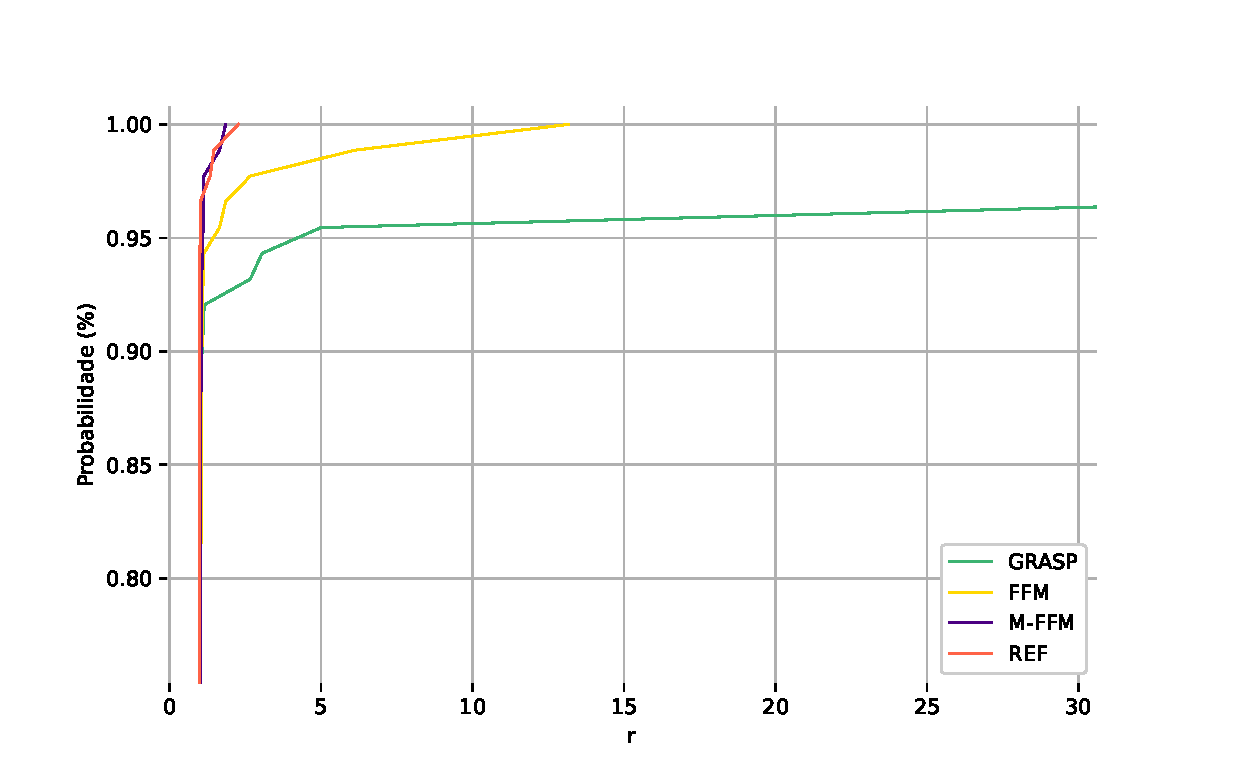
\includegraphics[width=0.3\textwidth]{figures/PP/PPGlobal.eps}
    }
    \subfloat[BBGRL]{
    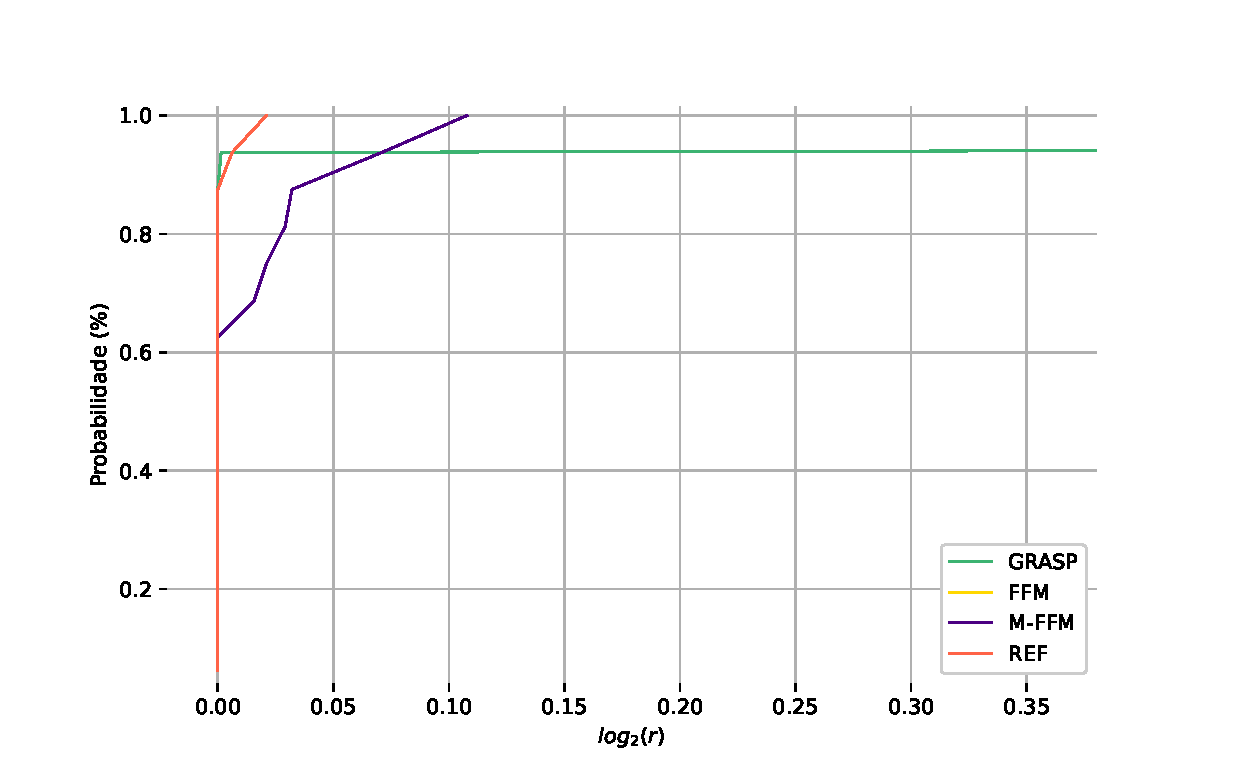
\includegraphics[width=0.3\textwidth]{figures/PP/PP_BBGRL.eps}
    }
    \qquad
    \subfloat[GBRL]{
    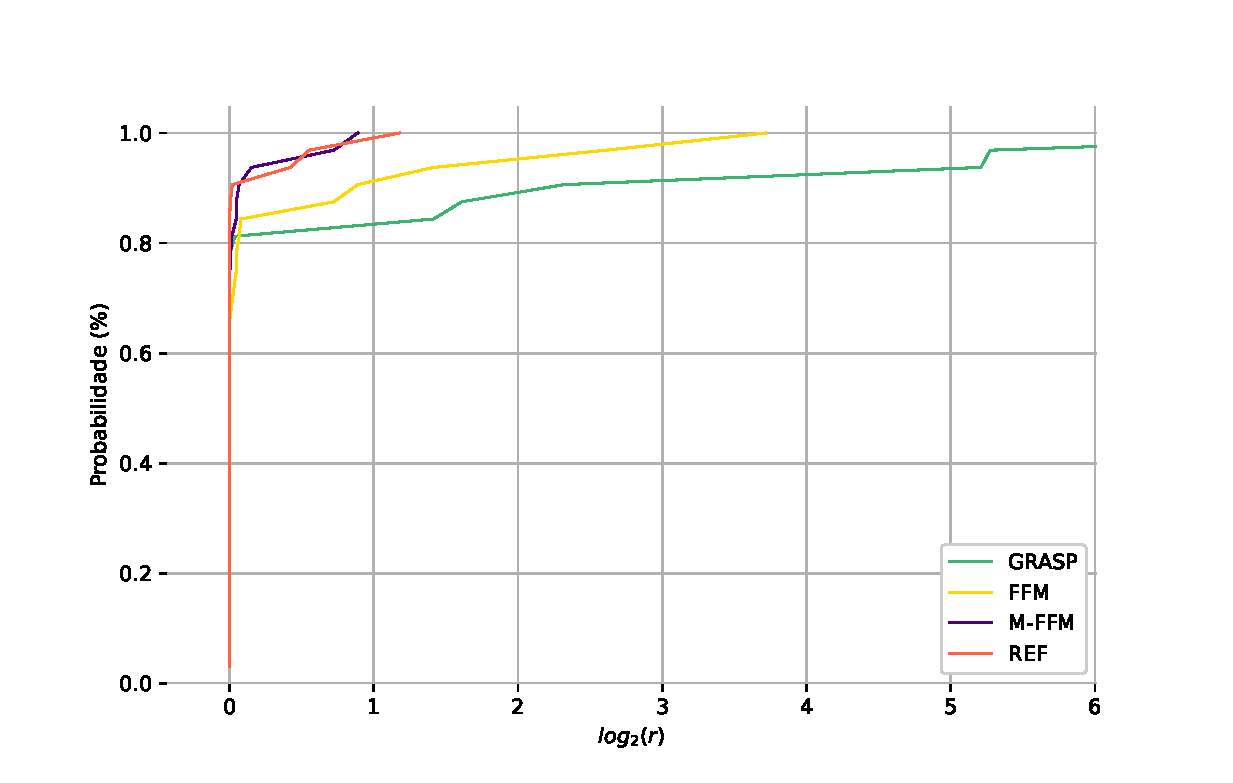
\includegraphics[width=0.3\textwidth]{figures/PP/PP_GBRL.eps}
    }
    \subfloat[GEN]{
    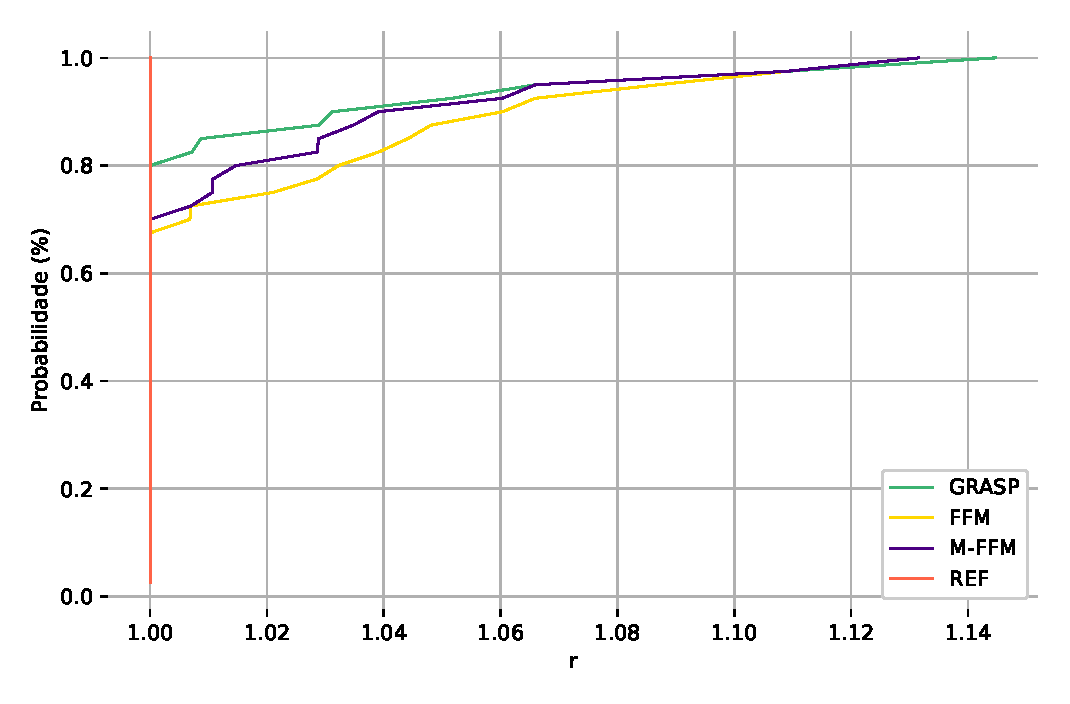
\includegraphics[width=0.3\textwidth]{figures/PP/PP_GEN.eps}
    }
    \caption{Perfis de Desempenho}
    \label{fig:pp}
\end{figure}

Os perfis confirmam os resultados observados em relação aos modelos: a curva do M-FFM domina a do FFM em todos os gráficos, ou ao menos se sobrepõe.

O perfil com o resultado mais interessante é o relacionado ao conjunto GEN. Neste, assim como nos outros, a referência possui os melhores resultados, mas as outras curvas seguem formatos similares, com a mateurística implementada claramente dominando as outras. O fato desse ser o único conjunto em que o incêndio se inicia sempre no vértice de maior grau confere uma maior dificuldade aos problemas a ser resolvidos e resulta em um desempenho melhor da mateurística em comparação aos outros.

No perfil relacionado ao conjunto BBGRL, é possível observar que a mateurística implementada superou a referência em algumas instâncias, mas em outras encontrou resultados de qualidade muito pior. Esse conjunto teve grande foco de instâncias nas quais os modelos não encontraram solução, o que explica o desempenho ruim.

Em geral, a mateurística teve um desempenho similar aos modelos, melhor em alguns casos e pior em outros. Porém, como já analisado, em certos casos a mateurística se destaca, como no caso do conjunto GEN. Como esperado, a implementação de referência, feita em C++ \cite{nat_dissertation} foi a que teve melhor desempenho. 

% Falar pelo menos sobre um exemplo interessante (tem caso que de 2 pra 4 bombeiros melhora drasticamente o resultado, ex: 1000_ep0.0075_0_gilbert_1.in)

\section{Conclusão}

    Como analisado, há uma clara relação entre alguns parâmetros do problema e a dificuldade desse. Apesar dos dados globais apontarem para uma aparente superioridade do modelo inteiro (em especial o M-FFM), a mateurística começa a se destacar conforme o problema se torna mais difícil, seja em instâncias grandes ou em casos em que há poucos bombeiros disponíveis. 

    Além disso, em todas as instâncias o foco do incêndio se iniciou em um único vértice, enquanto na realidade o fogo pode se espalhar antes mesmo de ser possível tomar alguma decisão. É razoável supor que nesses casos seja mais adequado resolver o problema com a mateurística - o perfil de desempenho do conjunto GEN revela que também há uma relação direta entre o conjunto $B$ e a dificuldade do problema. Para confirmar essa hipótese, seria interessante gerar novas instâncias com focos de fogo variados.
    
    Isto posto, o experimento foi um sucesso, atingindo resultados e comportamentos semelhantes à referência de Ramos et al. \cite{natanael}, mesmo não alcançando desempenho melhor na maioria das instâncias. Isso se deve ao grande número de diferenças na implementação, desde a mudança na ferramenta para solução dos modelos inteiros, até a linguagem de implementação.
    
    Além da implementação da mateurística descrita na Seção \ref{method}, houve a intenção de aproveitar os conceitos apresentados em outros métodos, baseados em metaheurísticas diferentes, como o \textit{Simulated Annealing} \cite{nat_dissertation}. Por questões de tempo, essas técnicas alternativas não foram implementadas, mas continuam sendo possíveis pontos para pesquisa futura, assim como o uso de \textit{path relinking}, exploração de caminhos entre soluções.

\bibliographystyle{ieeetr}
\small\bibliography{referencias}

\end{document}